\subsection{Central Velocity}

Throughout, though most obvious during H-burning, Mach number (\gls{Mach}) and \gls{ConvVel} modelled using \gls{MLT} increases steeply toward the centre, whilst those modelled using \gls{TDC} and those calculated using Equation \ref{eq:ManualVelocityCalc} (for both \gls{MLT} and \gls{TDC}) tend to zero (see Figure \ref{fig:MachMass_HBurn}).

This is surprising, since at such an early stage it is expected that, since timescales are long, $\texttt{MESA}$ will approximate \gls{TDC} as \gls{MLT}, meaning both values given for \gls{Mach} and \gls{ConvVel} would be equal (see Section \ref{sec:TDC}). 

This effect is likely caused by the differing treatment of conditions at the core: a difficult location to model in a 1D scenario. 

Notably, in a 3D model from \citet{Georgy24} \gls{ConvVel} values during Ne-burning appear to increase  toward the core (as implied by modelled \gls{MLT} values), though the overall profile shape should increase from a low, as predicted by \gls{TDC} and \gls{MLT} calculated with Equation \ref{eq:ManualVelocityCalc}.

The difference in treatment between values of \gls{ConvVel} and \gls{Mach} calculated and given by $\texttt{MESA}$ is further highlighted in Figure \ref{fig:MachMass_LateSiBurn}. Here, values calculated by $\texttt{MESA}$ appear to be a factor larger than those found using Equation \ref{eq:ManualVelocityCalc} for both mixing theories. 

This finding indicates Equation \ref{eq:ManualVelocityCalc} doesn't treat the envelope in the same way as by $\texttt{MESA}$, whilst showing envelope convection is treated similarly by both mixing theories. 

That said, values for \gls{TDC} and \gls{MLT} calculated by \texttt{MESA} are nearly equal in Figure \ref{fig:MachMass_LateSiBurn}, indicating treatment of \gls{ConvVel} is still similar, even at short timescales.

% \begin{figure*}[t]
% \centering
% \begin{subfigure}{0.7\textwidth}
%      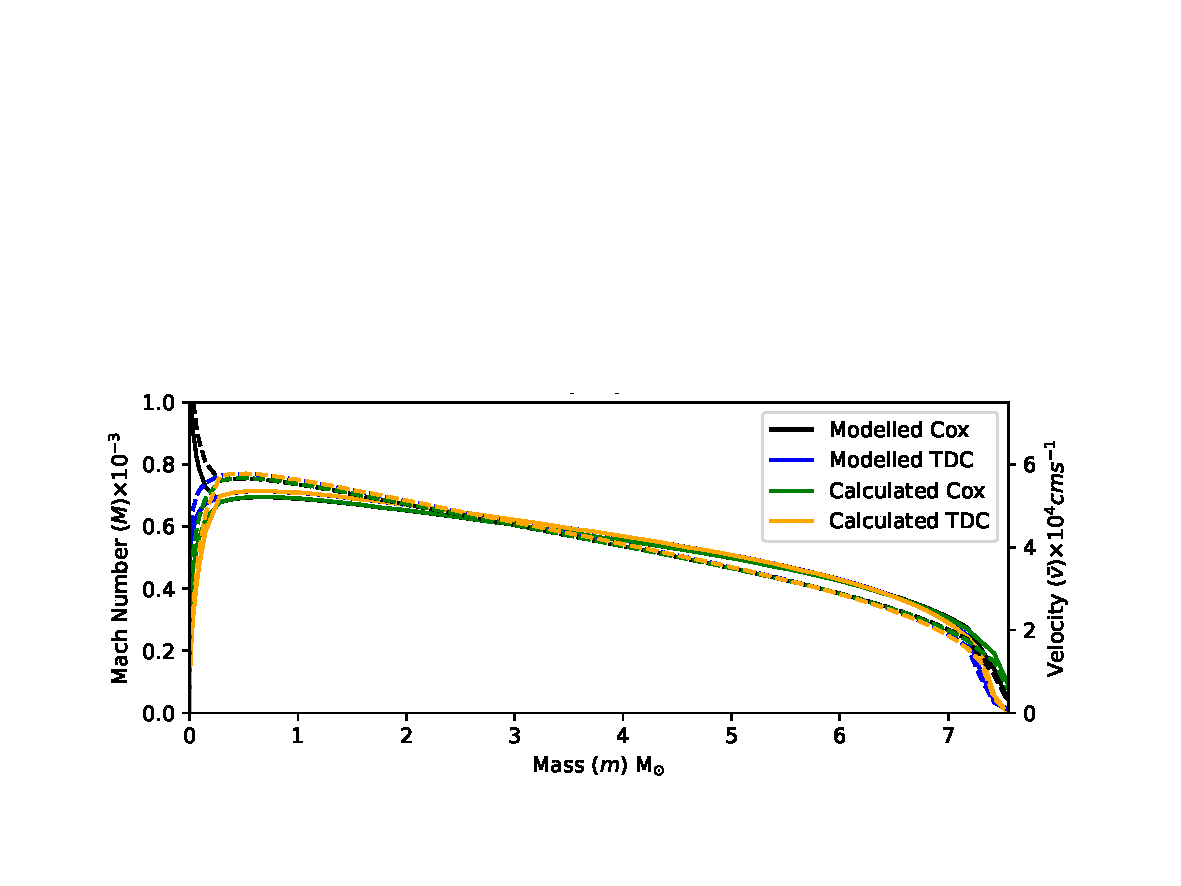
\includegraphics[width=\linewidth]{MachMass_HBurn}
%     \caption{Convection in the core region at $35\%$ core H to burn \\ ($\log \left(\text{time to core collapse}\right)$ is $\sim 6.41\mathrm{yr}$ for both models).}
%     \label{fig:MachMass_HBurn}
% \end{subfigure}

% \hfill
% \begin{subfigure}{\textwidth}
%     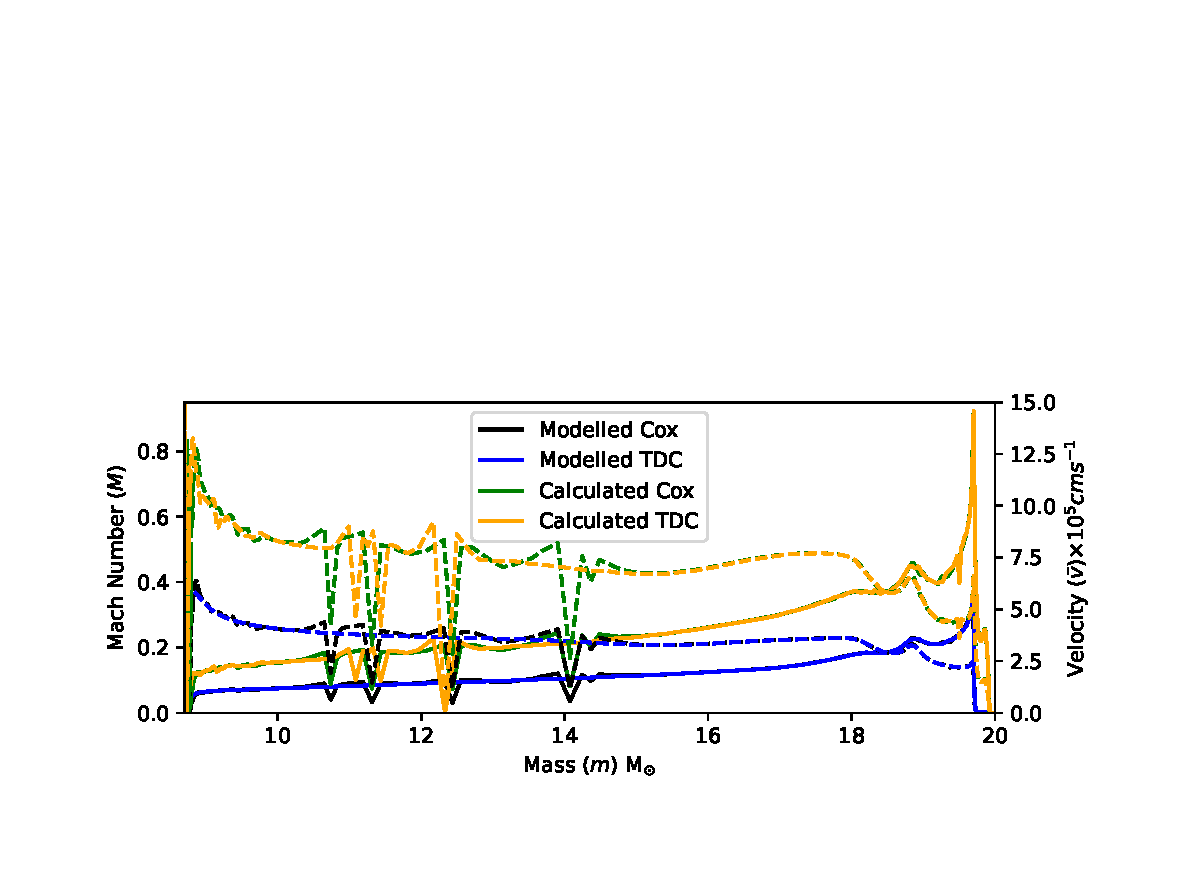
\includegraphics[width=\linewidth]{MachMass_EarlySiBurn}
%     \caption{Convection in the envelope at $95\%$ core Si to burn \\ ($\log \left(\text{time to core collapse}\right)$ is $\sim -2.44\mathrm{yr}$ for \gls{MLT} and $\sim -2.42\mathrm{yr}$ for \gls{TDC}).}
%     \label{fig:MachMass_EarlySiBurn}
% \end{subfigure}
% \hfill
% \begin{subfigure}{0.7\textwidth}
%      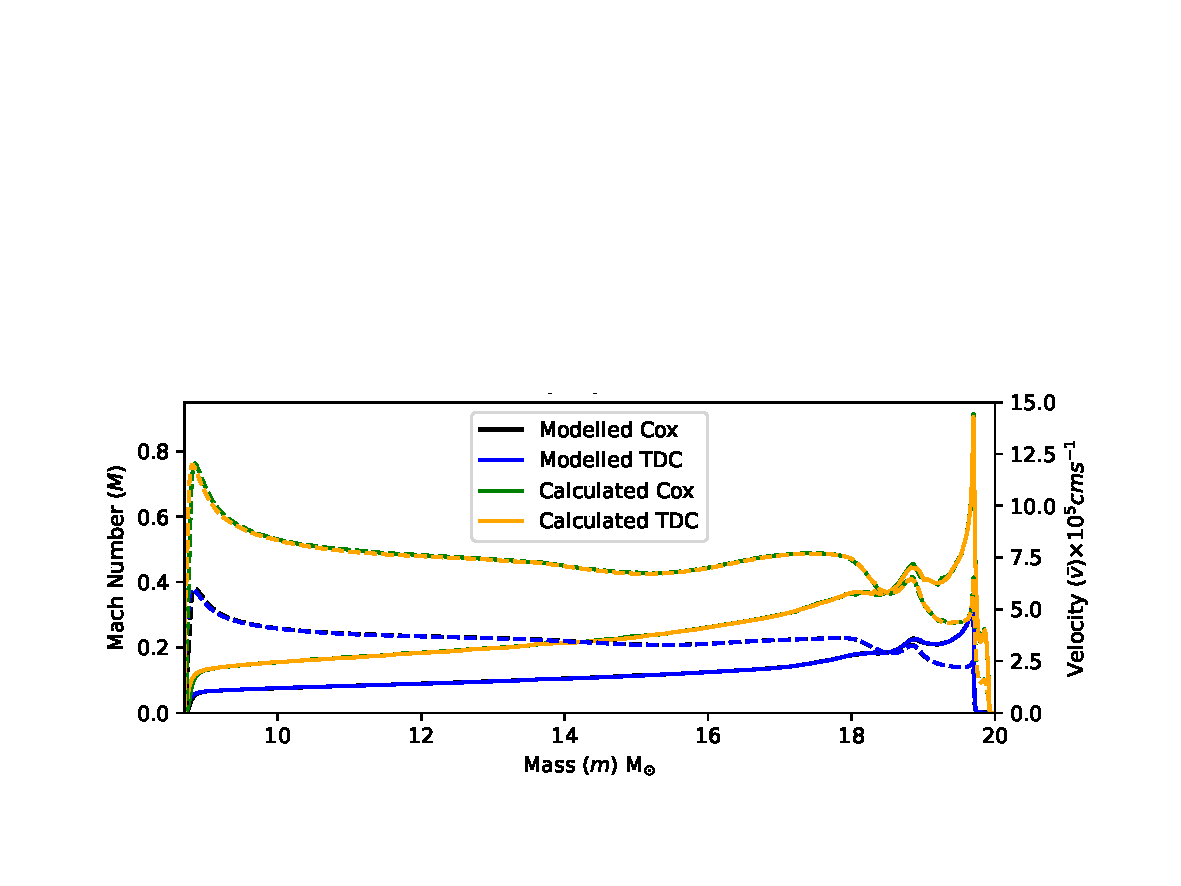
\includegraphics[width=\linewidth]{MachMass_LateSiBurn}
%     \caption{Convection in the envelope at $35\%$ core Si content during O-burning.}
%     \label{fig:MachMass_LateSiBurn}
% \end{subfigure}
% \caption{Graphs of Mach number and convective velocity by mass location. \textit{Modelled} pertains to the use of Equation \ref{eq:ManualVelocityCalc} and \textit{Calculated} to that directly calculated by \texttt{MESA}. Dashed lines are convective velocity measurements and full are of Mach number.}
% \label{fig:MachVel}
% \end{figure*}

% \begin{figure*}[t]   
% \centering
% 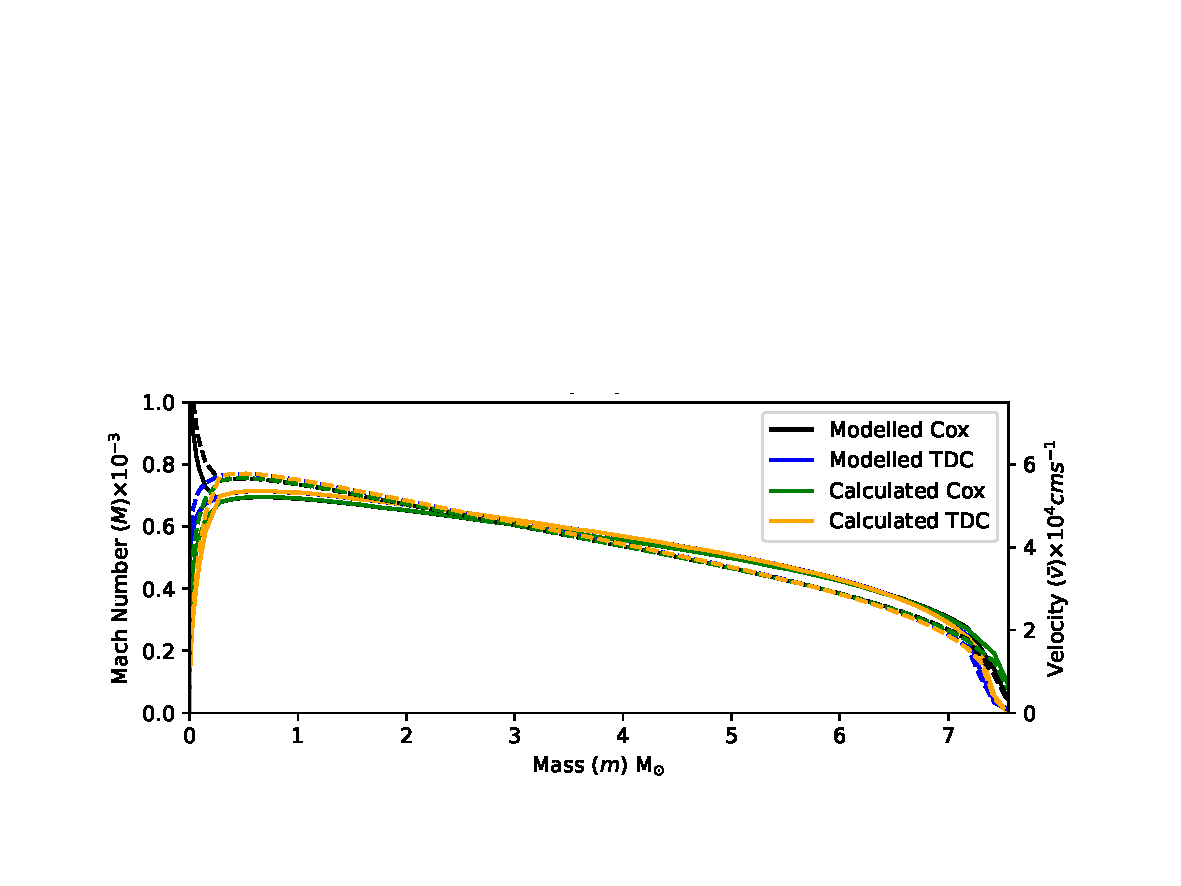
\includegraphics[width=0.8\linewidth]{MachMass_HBurn}
%     \caption{Graph of Mach number and convective velocity by mass location. \textit{Modelled} pertains to the use of Equation \ref{eq:ManualVelocityCalc} and \textit{Calculated} to that directly calculated by \texttt{MESA}. Dashed lines are convective velocity measurements and full are Mach number. Convection shown is in the core region at $35\%$ core H to burn ($\log \left(\text{time to core collapse}\right)$ is $\sim 6.41\mathrm{yr}$ for both models).}
%     \label{fig:MachMass_HBurn}
% \end{figure*}

%%%%%%
\begin{figure*}[t]
\centering
\begin{subfigure}{0.8\textwidth}
     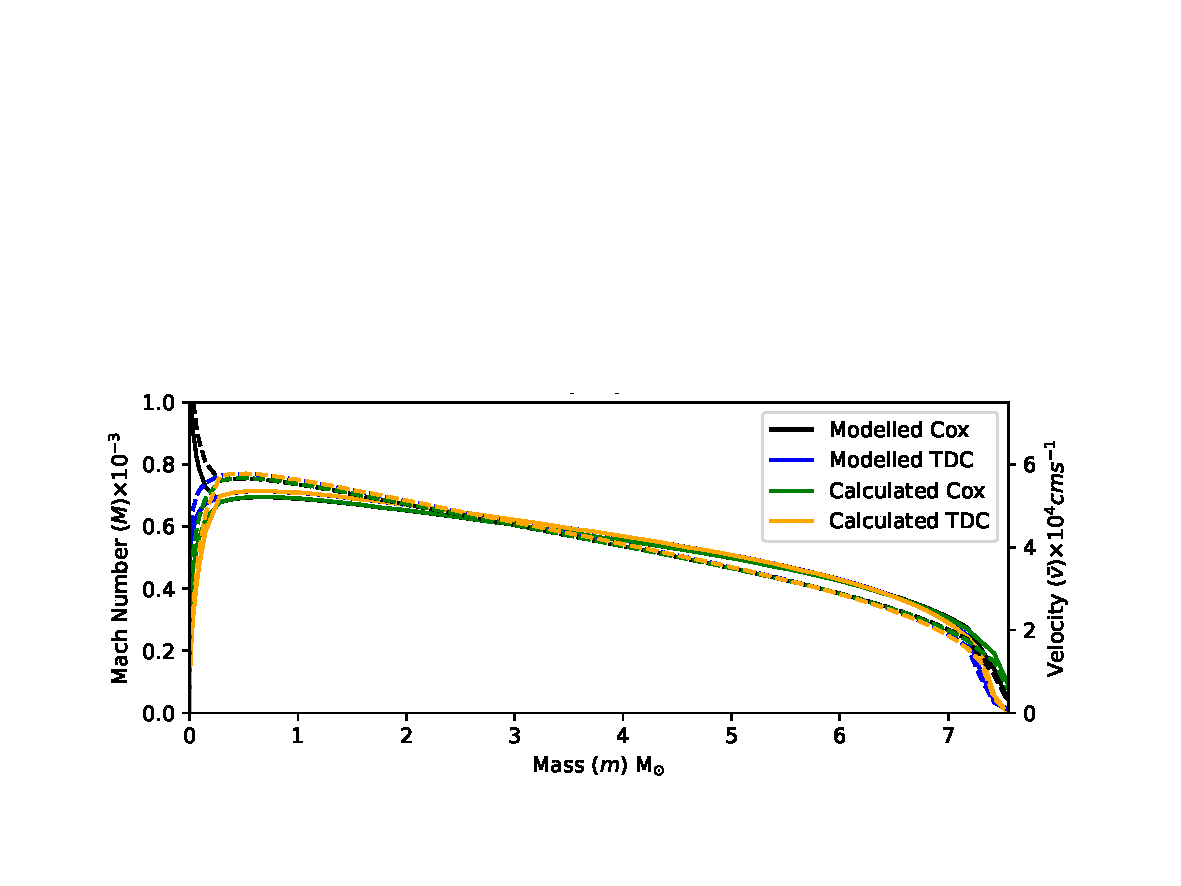
\includegraphics[width=\linewidth]{MachMass_HBurn}
    \caption{Convection shown is in the core region at $35\%$ core H to burn ($\log \left(\text{time to core collapse}\right)$ is $\sim 6.41\mathrm{yr}$ for both models).}
    \label{fig:MachMass_HBurn}
\end{subfigure}
\hfill
\begin{subfigure}{0.8\textwidth}
    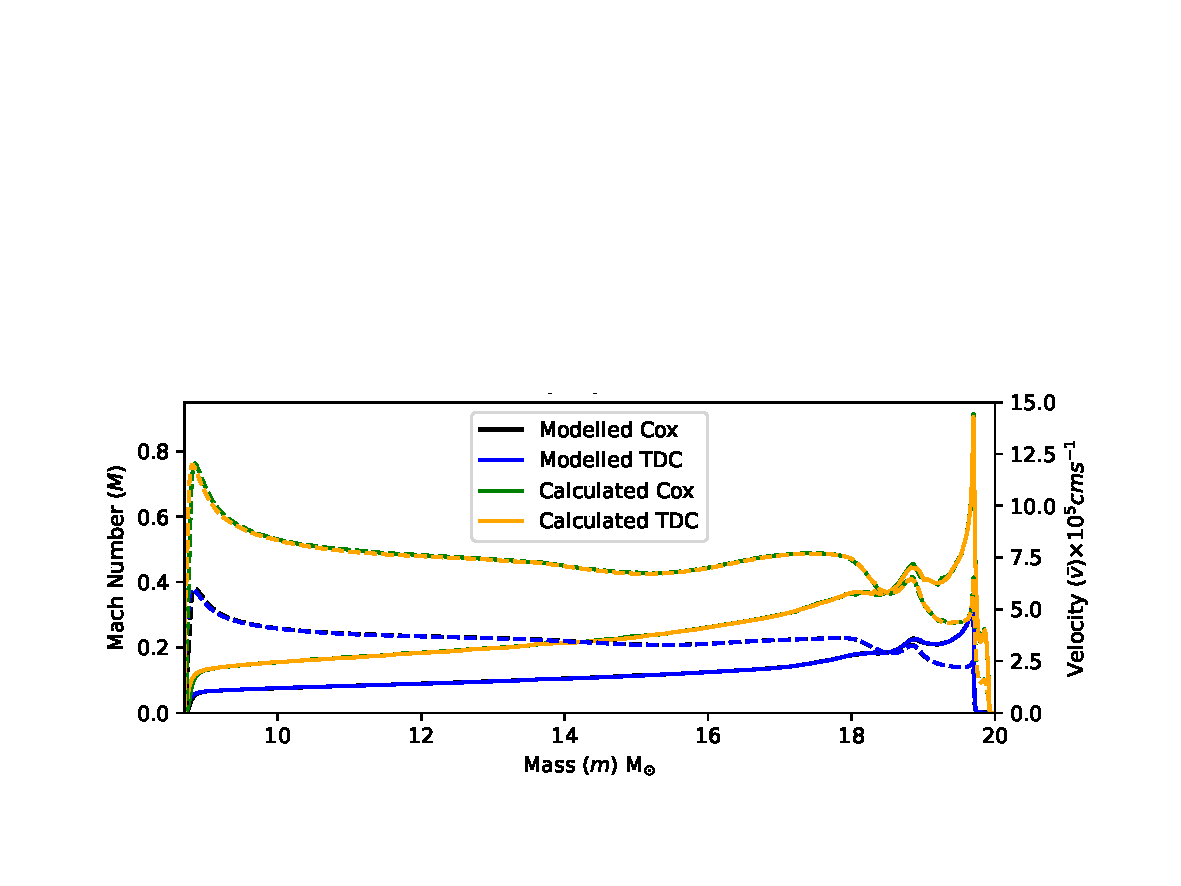
\includegraphics[width=\linewidth]{MachMass_LateSiBurn}
    \caption{Convection in the envelope during O burn, close to core collapse. ($\log \left(\text{time to core collapse}\right)$ is $\sim -0.35\mathrm{yr}$ for \gls{MLT} and $\sim -0.38\mathrm{yr}$ for \gls{TDC}).}
    \label{fig:MachMass_LateSiBurn}
\end{subfigure}
% \hfill
% \begin{subfigure}{0.7\textwidth}
%      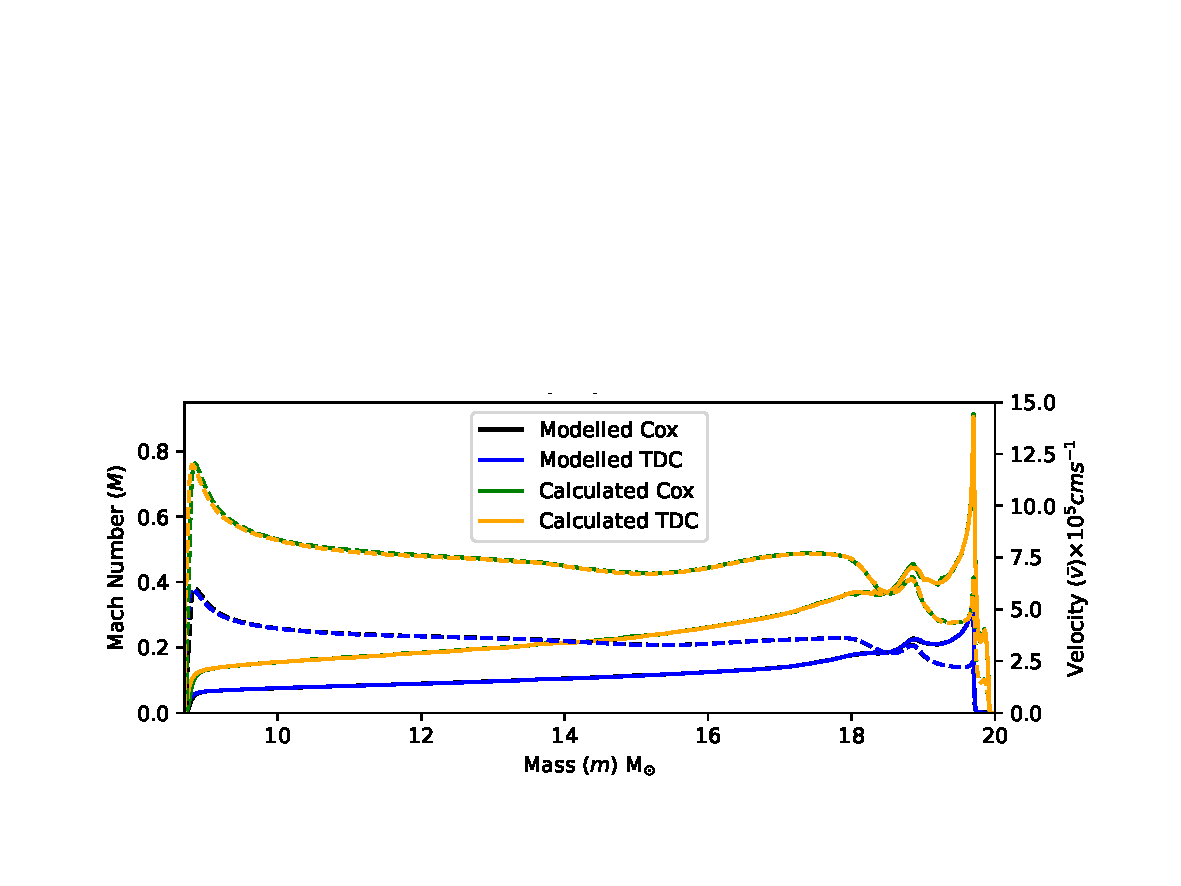
\includegraphics[width=\linewidth]{MachMass_LateSiBurn}
%     \caption{Convection in the envelope at $35\%$ core Si content during O-burning.}
%     \label{fig:MachMass_LateSiBurn}
% \end{subfigure}
\caption{Graphs of Mach number and convective velocity by mass location. \textit{Modelled} pertains to the use of Equation \ref{eq:ManualVelocityCalc} and \textit{Calculated} to that directly calculated by \texttt{MESA}. Dashed lines are convective velocity measurements and full are Mach number.}
\label{fig:MachVel}
\end{figure*}